\documentclass[a4paper]{article}
\usepackage[english]{babel}
\usepackage[utf8x]{inputenc}
\usepackage[T1]{fontenc}
\usepackage[a4paper,top=4cm,bottom=3cm,left=4cm,right=4cm,marginparwidth=1.95cm]{geometry}

\usepackage{xcolor}
\usepackage{amsmath}
\usepackage{graphicx}
\usepackage{mathtools}
\usepackage{titlesec}
\titleformat{\subparagraph}
    {\normalfont\normalsize\bfseries}{\thesubparagraph}{1em}{}
\titlespacing*{\subparagraph}{\parindent}{3.25ex plus 1ex minus .2ex}{.75ex plus .1ex}

\title{Latex - Referat}
\author{Cezary Krysztoszek}

\begin{document}
\maketitle 

\section{Rozdzial numerowany}
\subparagraph{Podpunkt numerowany}

\section*{Rozdzial nienumerowany}
\subparagraph*{Podpunkt}
\section {Numerowanie}
\begin{enumerate}
\item Pierwszy
\item Kolory \newline
{\color{red} Troche czerwonego} \newline % zalamanie lini
\emph{Tekst na czarno {\color{blue} Troche niebieskiego} i na koniec znowu czanry}
\end{enumerate}
\section{Tabela}
\begin{tabular}{|r|l r|}  % okresla jakiej szerokosci bedzie tabela oraz ich format r-right(prawo stronne, l-left(lewo stronny), c - centrum. Pionowe kreski reprezentują linie między tabelami
  \hline 
  pozycja 11 & pozycja 12 & pozcja 13\\
  \hline
  pozycja 21 & pozycja 22 & pozycja 23 \\
  \hline % reprezentuje dolną linie
  pozycja 31 & pozycja 32 
  
\end{tabular} 
\section{Obrazki}
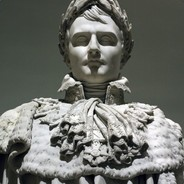
\includegraphics[width=5cm, height=5cm]{obrazek1}
\newpage % kolejna strona
\section{Matematyka}
\begin{math}
\alpha, \beta,  \gamma
\cos (2/\alpha), \sin (45^\circ )
\end{math}
\subparagraph{Potęgi i Pierwiastki, i Index Dolny}

$$ \sqrt{25} = 5 $$
$$ 3^2 = 9 $$
$$ k_0 + k_1 + ... + k_{n+1} $$ % przy dłuższych(większych niż 1 symbool) indexach dolnych i górnych należy używać nawiasów klamrowych.

\subparagraph{Ułamki}
$ \frac{25}{5} = 5 $ \newline
$ \frac{\frac{3}{6}}{123} $
\subparagraph{Operacje na zbiorach}
\begin{tabular}{| r | r |}
\hline
Symbol & Kod \\
\hline
$ \subset $ & subset \\
\hline
$ \subseteq $ & subseteq \\
\hline
$ \supset $ & supset \\
\hline
$ \supseteq $ & supseteq \\
\hline 
$ \times $ & times \\
\hline
\end{tabular}
\subparagraph{Logika}
\begin{tabular}{|r|r|}
\hline
Symbol & Kod \\
\hline
$ \neg $ & neg \\ % negacja
\hline
$ \implies $ & implies \\ % implikacja
\hline
$ \iff $ & iff \\ % rownowaznosc
\hline
$ \land $ & land \\	% koniunkacja	
\hline 
$ \lor $ & lor \\ % alternatywa
\hline
\end{tabular}
\subparagraph{Macierze}
\begin{math}
\begin{bmatrix}
       \frac{3}{7} & \frac{1}{6} & \frac{1}{4} \\[0.3em]
       \frac{5}{6} & 0           & \frac{5}{6} \\[0.3em]
       0           & \frac{5}{21} & \frac{1}{6}
     \end{bmatrix} 
\end{math}







\end{document}